\section{Result Evaluation}
\label{chap:6}
Regarding the network topologies, ten different topologies were generated with the Stochastic Block Model for $n = 64, 256, 512,..., 32768$. The number of blocks $k$ was set to $\log n$. The values were set to $p = 7{\tfrac {\ln n}{n}}$ for the diagonal of the probability matrix and  $p\prime = {\tfrac {10}{n}}$ for values out of the diagonal. The values for the parameters are similar to the values used in \cite{kothapalli2013analysis}.

First, the result of the evaluation of the \textit{MIS} algorithm are presented. Then, the analysis of the synchronisation techniques and finally the conclusion of the evaluation.

% The results presented are the average of 10 executions of the simulation for each topology. For the \textit{MIS} algorithm it is important to measure the average of the execution because the algorithm is randomised and the unpredictable behaviour of the asynchronous message passing at the bottom. In consequence, for a given topology it is possible to obtain different results. The results observed in the simulation show that the number of rounds is similar in different execution however in can be some important differences in the number of messages. These results are presented in the next section.


\subsection{Evaluation of MIS algorithm}

The figure \ref{fig:rounds_execution} shows the average number of round that takes on each topology to finish the \textit{MIS} algorithm. As seen in section \ref{cap:2}, the expected termination time of the algorithm is $O(\log N)$ rounds. The plot is compared with a logarithmic plot showing similarity in shape of curves.The figure \ref{fig:rounds-erdos} shows the average number of round per topology using network topologies generated by the Erd\~os--R\'enyi model with  $p = 5{\tfrac {\ln n}{n}}$. The shape of the curve also is similar to the logarithmic curve shape for graphs with a constant probability distribution of edges.


\begin{figure}[ht]
\centering
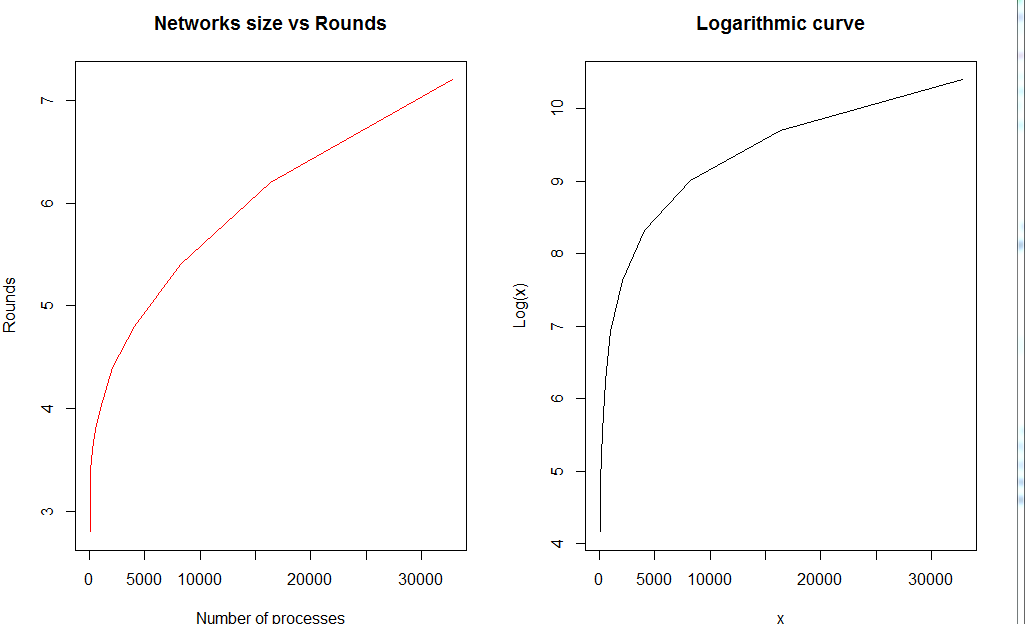
\includegraphics[width=1 \linewidth, height=6cm]{number_rounds.png} 
\caption{Rounds per execution vs log(x) curve}
\label{fig:rounds_execution}
\end{figure}



\begin{figure}[ht]
\centering
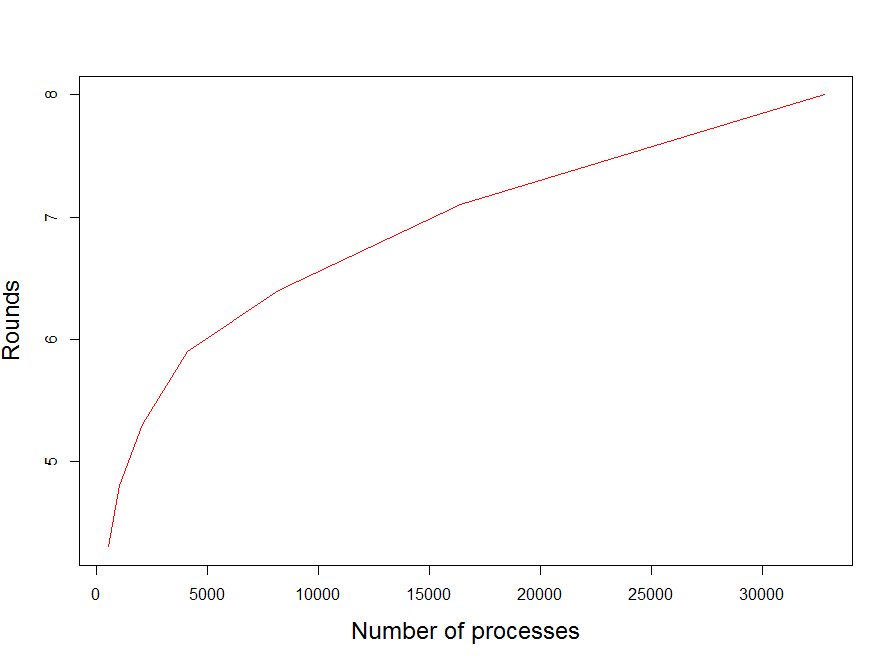
\includegraphics[width=1 \linewidth, height=8cm]{execution-rounds-erdos.PNG} 
\caption{Rounds of MIS algorithm using Erdos-Renyi model for network topologies}
\label{fig:rounds-erdos}
\end{figure}


The distributed algorithm should make a progression in each round on the number of processes that finish the local algorithm and become inactive according to the proof of termination in \cite{yves2009optimal}. This progression for a network of 32768 processes can be seen in the figure \ref{fig:progression} . The blue line represents the number of processes that join the \textit{MIS}  per round and the red line represents the number the neighbours of some process that took part of the \textbf{MIS}. The figure \ref{fig:actives}, shows the total number of processes that are active in each round for the same execution. By the end of round 14, the network has no active processes.  

\begin{figure}[ht]
\centering
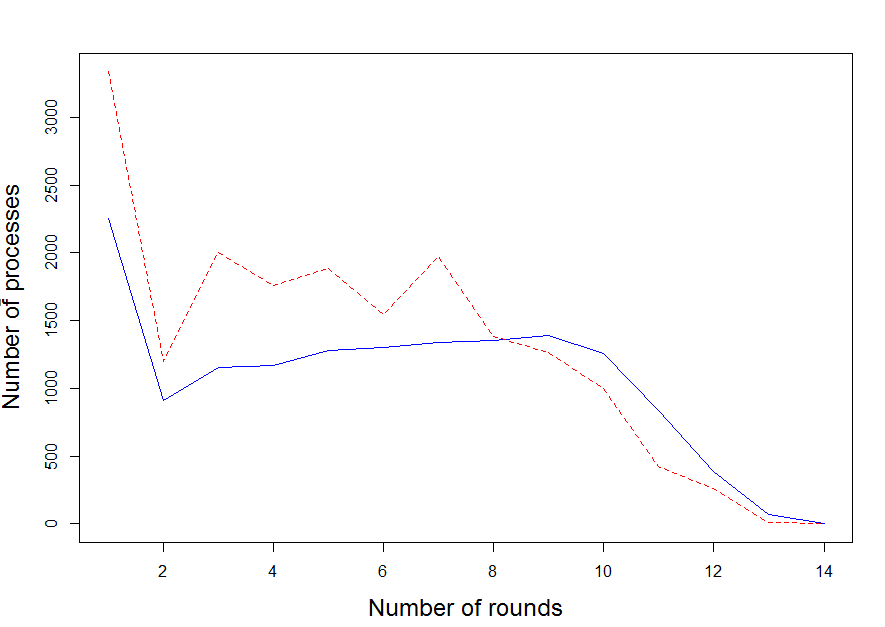
\includegraphics[width=1 \linewidth, height=8cm]{progress.PNG} 
\caption{Numbers of processes that finish the execution per round (MIS and not MIS)}
\label{fig:progression}
\end{figure}

\begin{figure}[ht]
\centering
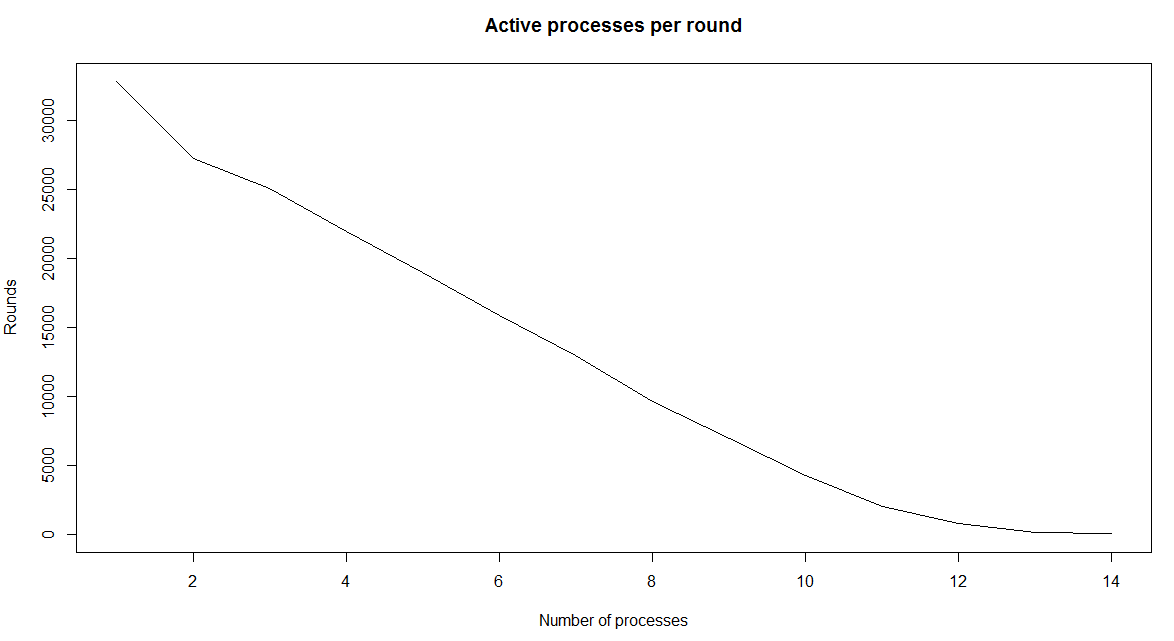
\includegraphics[width=1 \linewidth, height=8cm]{actives_round.PNG} 
\caption{Total numbers of processes that finish the execution per round}
\label{fig:actives}
\end{figure}


\subsection{Evaluation of Synchronizers}

To evaluate the messages send by the algorithm first, we need to make a distinction between messages sent by the synchronous algorithm and the additional messages send by the synchronizers. In the case of Alpha and Beta, it is straightforward to count this two types of messages. Every time a process use the \textbf{sync-send} function, it is count as one message sent by the algorithm. For every synchronous message, the synchronizer sends some asynchronous messages which are multiple of its neighbour size and also depend on the mechanism used to detect when a process is safe. For the Global synchronizer, the counting is a little more complicated. The messages for acknowledgement, to update the topology and the notifications to the master process count as synchronisation overhead.


The figure \ref{fig:total_msg} illustrate the messages send by each synchronizer for the network of 32768 processes. The orange bar represents the synchronisation overhead and the blue bar the messages sent by the synchronous algorithm. It is clear that the global synchronizer is the one with the best performance. In this case, the synchronisation adds around $20 \%$ more messages. For the other two, the difference is overwhelming. The reason is that the Global synchronizer is optimal concerning the messages send by actives processes. In each round, once a process becomes inactive, no additional messages are sent by this process. On the contrary, Alpha and Beta require the entire topology to participate in every round until the distributed algorithm end.  The figure \ref{fig:total_msg-round} shows how the number of messages decreases in each round for the global synchronizer, however, for Alpha and Beta remain constant. Finally, the figure \ref{fig:total_msg-size} shows the total number of messages send by the algorithm for different networks size. The messages complexity is bounded by the number of edges of the topology and a constant factor. The three functions show an approximate the shape of a line in agreement with the theoretical analysis.





\begin{figure}[ht]
\centering
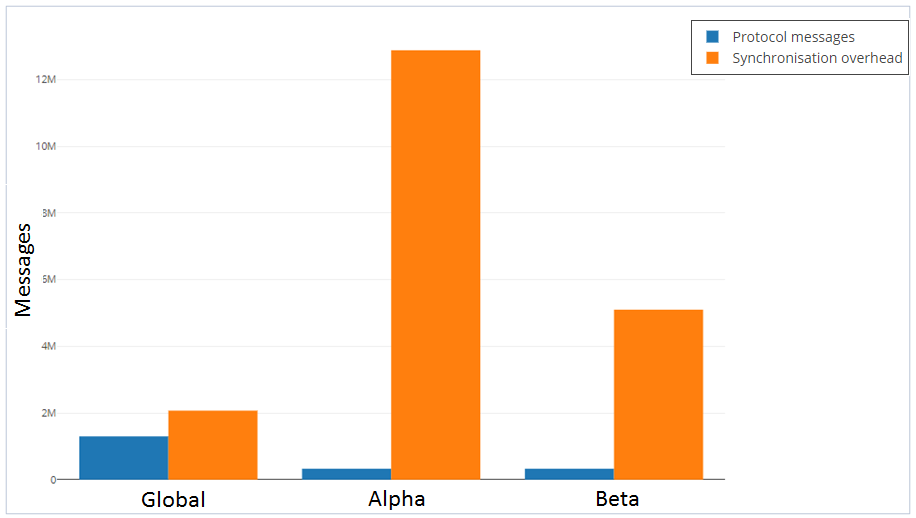
\includegraphics[width=1 \linewidth, height=7cm]{messages-synchroniser1.PNG} 
\caption{Messages send by the algorithm and Synchronizer}
\label{fig:total_msg}
\end{figure}

\begin{figure}[ht]
\centering
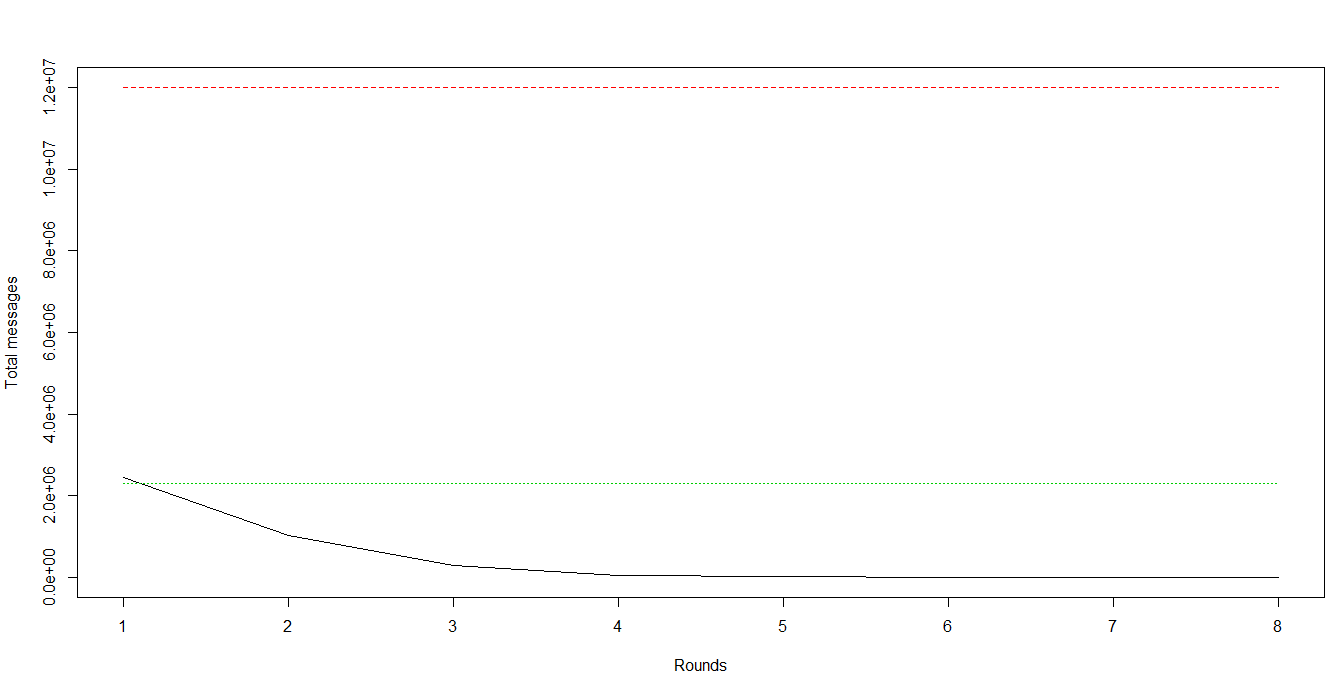
\includegraphics[width=0.9 \linewidth, height=6cm]{messages-rounds.PNG} 
\caption{Messages send by the algorithm in different rounds}
\label{fig:total_msg-round}
\end{figure}

\begin{figure}[ht]
\centering
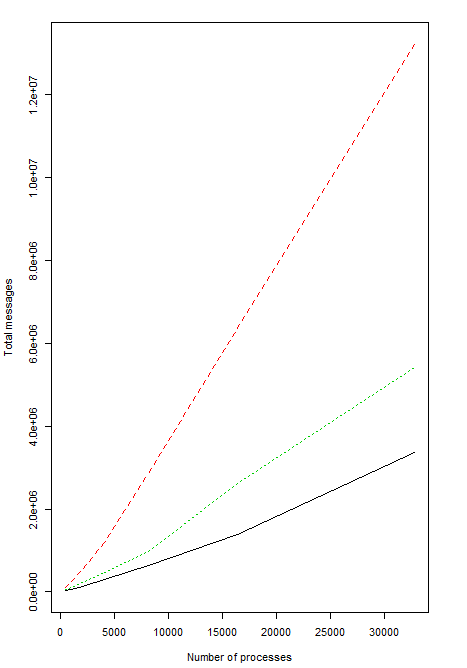
\includegraphics[width=0.8 \linewidth, height=6cm]{messages-network.PNG} 
\caption{Total Messages vs Network size}
\label{fig:total_msg-size}
\end{figure}


\subsection{Conclusions}

In this dissertation, the problem of finding the Maximal Independent Set in general graphs was studied. Distributed algorithms provide better time complexity than sequential algorithm.  A distributed synchronous algorithm was implemented in order to analyse time and message complexity for the \textit{MIS} problem. Synchronous algorithms are easy to design and have lower complexity than asynchronous ones.

\newpage
